\documentclass[11pt,letterpaper]{article}
\usepackage[margin=0.9in]{geometry}
\usepackage[T1]{fontenc}
\usepackage[utf8]{inputenc}
\usepackage{lmodern,microtype}
\usepackage{enumitem,booktabs,tabularx,longtable}
\usepackage{amsmath,amssymb}
\usepackage{tikz}
\usepackage{xcolor}
\usepackage{pdfpages}
\usepackage[hidelinks]{hyperref}
\setlength{\parskip}{.48em}
\newcommand{\AuthorExact}{\textless Brian Tenneson\textgreater}
\newcommand{\EditorialFooter}[1]{%
\begin{tikzpicture}[remember picture,overlay]
\node[anchor=south west,inner sep=0pt] at ([xshift=74pt,yshift=13pt]current page.south west) {\sffamily\fontsize{7}{8}\selectfont\color{black!72}\textbf{X0 retrospective citation:} #1};
\end{tikzpicture}}
\begin{document}
\pagenumbering{roman}
\begin{center}
{\LARGE\bfseries X0: Formal Self-Awareness in Semi-Ideal Computers}\\[8pt]
{\large Citation-added, explicitly attributed edition of immutable W0}\\[7pt]
\AuthorExact\\[7pt]
\textit{Editorial edition: October 31, 2026. Original expanded draft: October 28, 2026.}
\end{center}
\par\noindent\emph{See the AI disclaimer that follows this essay.}\par\medskip
\noindent\fcolorbox{black!45}{black!3}{\begin{minipage}{0.94\linewidth}
\textbf{Priority and attribution declaration.} X0 reproduces nineteen W0-derived pages from the recovered original W0 LaTeX source, with Figures 2--4 editorially repaired to avoid overlapping labels. The original W0 source is preserved separately and the mathematics is unchanged. This X0 edition adds retrospective citations and original-source-page navigation. This front matter, the small editorial citation markers, and the bibliography are \emph{retrospective scholarly additions}. They explicitly acknowledge established work; they do not imply that W0's author discovered or first proved classical results, nor that those references were consulted when W0 was drafted. The historical author credit remains as supplied, and W0 itself is not overwritten. \textbf{This is not a formal verification or an exhaustive originality audit.}
\end{minipage}}\par\medskip
\noindent\textit{Formal Self-Awareness Trilogy --- Part I of III; publication-preparation repair, October 31, 2026.}\par\medskip
\section*{How to read claims of originality}
\textbf{Established prior concepts:} self-reference and formal provability \cite{godel,lob,feferman}; future-state equivalence and behavioral simulation \cite{nerode,milner}; independently checkable proof evidence \cite{necula,besson}; and Tegmark's philosophical self-aware-substructure hypothesis \cite{tegmark}. These subjects predate W0 and are not claimed as originating with its author.

\textbf{W0-specific formulation:} the notation of xyz formal systems and semi-ideal computers, the distinguished tag-and-self-theory conventions, the operational interpretation of nested self-claims, and conditional transfer lemmas are presented as a \emph{specialized framework}. A mathematical proof of a statement in that framework does not certify that the underlying general principle is historically new.

\textbf{No consciousness claim:} W0 studies formal statements, derivations, histories, and simulations. Its definitions should not be read as a demonstration of experience, intelligence, or subjective awareness.
\noindent\textbf{Diagram repair note.} In this edition, W0 Figures 2, 3, and 4 are typeset with adjusted TikZ geometry to prevent overlapping labels. Original W0 LaTeX source is archived unchanged as a separate file; mathematical prose, theorem statements, and arguments have not been altered.\par\medskip
\noindent\textbf{Citation key (two distinct namespaces).} The numbered references \textbf{[1]--[4]} appearing in the source's original ``Source note and references'' section identify historical W0 source notes and have not been renumbered or reinterpreted. Citations of the form \textbf{[E1]--[E8]} throughout this editorial front matter, on source-page footers, and in the editorial back matter refer \emph{only} to the retrospective X0 editorial bibliography. They are not claims about sources consulted in the original W0 writing.\par\medskip
\clearpage
\section*{Section-by-section prior-art map}
\small
\begin{longtable}{@{}p{0.22\linewidth}p{0.74\linewidth}@{}}
\toprule Original W0 pages & Earlier concepts and corresponding references \\\midrule
1--4 & Self-reference and formal logical systems \cite{godel,lob,feferman}; machines, equivalence, and simulation as broader traditions \cite{nerode,milner}. \\
5--8 & Machine names, quotation, operational self-ascription, and reflection: prior provability work \cite{godel,lob,feferman}; proof checker caveat \cite{necula}. \\
9--12 & Reflection and deterministic simulation: established equivalence and simulation techniques \cite{nerode,milner}; W0's added tag/quotation/certificate hypotheses are specialized modeling assumptions. \\
13--16 & Branching process comparisons and evidence-preserving histories: precedents in behavioral semantics \cite{milner} and proof-carrying certificates \cite{necula,besson}. \\
17 & The ``self-aware substructure'' philosophical motivation belongs to Tegmark \cite{tegmark}; W0's technical criterion does not prove any consciousness claim. \\
18--19 & Open questions and W0 source notes are future directions, not established novelty; classical theory remains appropriately attributed above. \\
\bottomrule
\end{longtable}
\normalsize
\clearpage
\phantomsection
\pdfbookmark[1]{Editorial contents and page guide}{x0contents}
\section*{Contents and page-number guide}
\noindent\small This is an editorial navigation guide to the retained nineteen W0-derived source pages. The source's original table of contents appears on \textbf{PDF pages 4--5}, and its page numbers restart at \textbf{1}. The table below gives both the original \textbf{W0 page} and the actual \textbf{PDF page} so that no page-number conversion is needed. Each title is a clickable link.\par\medskip
\renewcommand{\arraystretch}{1.15}
\setlength{\tabcolsep}{3pt}
\footnotesize
\begin{tabularx}{\linewidth}{@{}rXrr@{}}
\toprule
\# & Section (click to navigate) & W0 page & PDF page \\
\midrule
\textbf{1} & \hyperlink{w0p3}{Introduction: what is the claim?} & 3 & 6 \\
\textbf{2} & \hyperlink{w0p3}{The xyz language and the SIC layer} & 3 & 6 \\
\textbf{3} & \hyperlink{w0p5}{Internal representations and self-theories} & 5 & 8 \\
\textbf{4} & \hyperlink{w0p6}{Awareness predicates and the first examples} & 6 & 9 \\
\textbf{5} & \hyperlink{w0p7}{Quotation, provability, and the reflection sequence} & 7 & 10 \\
\textbf{6} & \hyperlink{w0p8}{Existence, strictness, and non-degenerate reflection} & 8 & 11 \\
\textbf{7} & \hyperlink{w0p9}{Self-awareness and the simulation preorder} & 9 & 12 \\
\textbf{8} & \hyperlink{w0p12}{Two depths, two time scales, and their relation} & 12 & 15 \\
\textbf{9} & \hyperlink{w0p13}{Nondeterminism: may, must, and the fairness boundary} & 13 & 16 \\
\textbf{10} & \hyperlink{w0p14}{History, provenance, and safe compression} & 14 & 17 \\
\textbf{11} & \hyperlink{w0p15}{A worked model: a prover that proves its own kind} & 15 & 18 \\
\textbf{12} & \hyperlink{w0p15}{Cooperative ATPs and AMLD-style self-description} & 15 & 18 \\
\textbf{13} & \hyperlink{w0p16}{Tegmark's self-aware substructures: a controlled comparison} & 16 & 19 \\
\textbf{14} & \hyperlink{w0p17}{What has been shown, what has not, and future research} & 17 & 20 \\
\textbf{15} & \hyperlink{w0p18}{Conclusion} & 18 & 21 \\
\midrule
 & \hyperlink{w0p18}{Source notes and references} & 18 & 21 \\
 & \hyperlink{editorialback}{Editorial attribution and bibliography} & -- & 23 \\
 & \hyperlink{disclaimer}{AI disclaimer} & -- & 24 \\
\bottomrule
\end{tabularx}
\normalsize
\par\medskip
\noindent\footnotesize\textbf{Provenance.} The source pages were compiled from W0 LaTeX with editorially repaired Figures 2--4. This navigation guide changes no source mathematics or diagram. All E-prefixed citations remain retrospective editorial attributions. The unmodified original W0 LaTeX is included alongside the editorial figure edition.\normalsize
\clearpage
\pagenumbering{arabic}
\setcounter{page}{1}
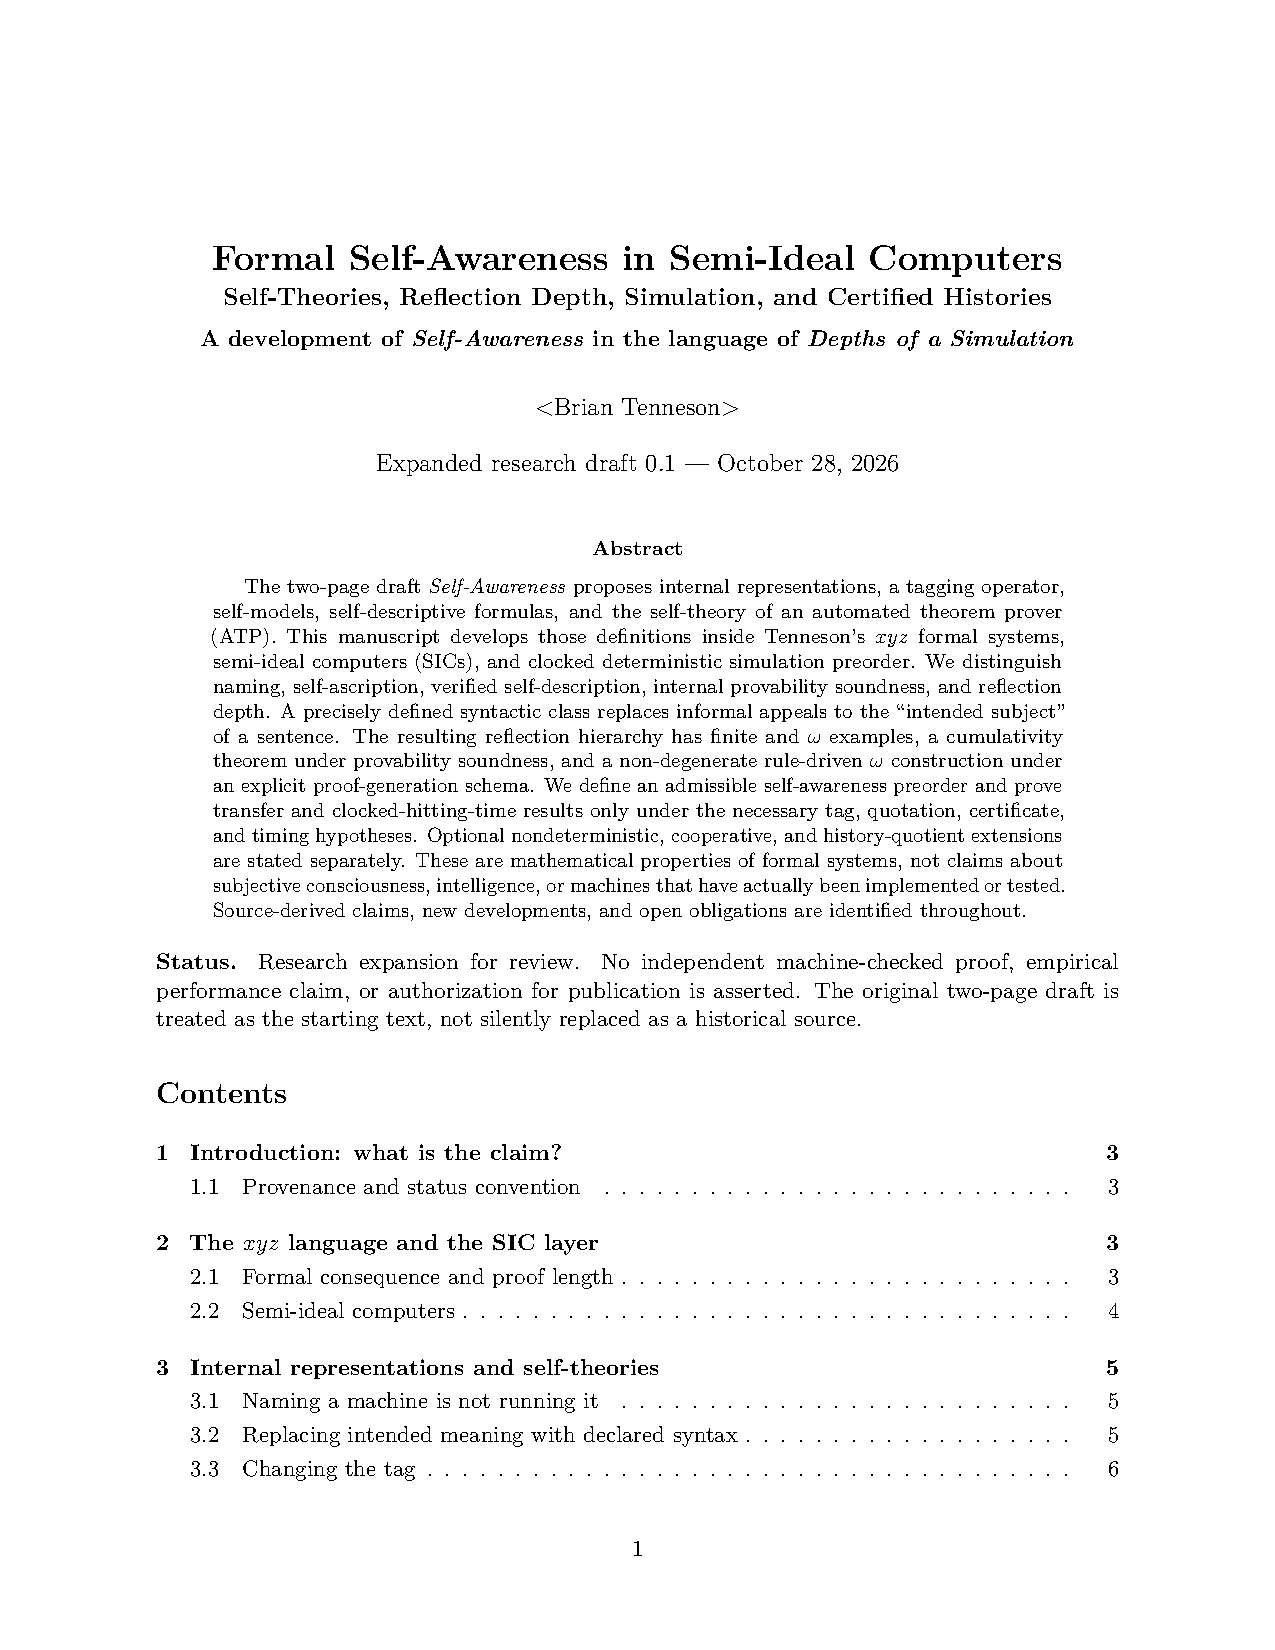
\includepdf[pages={1},pagecommand={\thispagestyle{empty}\hypertarget{w0p1}{}\EditorialFooter{\cite{godel,lob,feferman}}}]{W0_Editorial_Figures_Repaired.pdf}
\includepdf[pages={2},pagecommand={\thispagestyle{empty}\hypertarget{w0p2}{}\EditorialFooter{\cite{godel,lob,feferman}}}]{W0_Editorial_Figures_Repaired.pdf}
\includepdf[pages={3},pagecommand={\thispagestyle{empty}\hypertarget{w0p3}{}\EditorialFooter{\cite{godel,nerode,milner}}}]{W0_Editorial_Figures_Repaired.pdf}
\includepdf[pages={4},pagecommand={\thispagestyle{empty}\hypertarget{w0p4}{}\EditorialFooter{\cite{nerode,milner}}}]{W0_Editorial_Figures_Repaired.pdf}
\includepdf[pages={5},pagecommand={\thispagestyle{empty}\hypertarget{w0p5}{}\EditorialFooter{\cite{godel,lob}}}]{W0_Editorial_Figures_Repaired.pdf}
\includepdf[pages={6},pagecommand={\thispagestyle{empty}\hypertarget{w0p6}{}\EditorialFooter{\cite{godel,necula}}}]{W0_Editorial_Figures_Repaired.pdf}
\includepdf[pages={7},pagecommand={\thispagestyle{empty}\hypertarget{w0p7}{}\EditorialFooter{\cite{godel,lob,necula}}}]{W0_Editorial_Figures_Repaired.pdf}
\includepdf[pages={8},pagecommand={\thispagestyle{empty}\hypertarget{w0p8}{}\EditorialFooter{\cite{lob,feferman}}}]{W0_Editorial_Figures_Repaired.pdf}
\includepdf[pages={9},pagecommand={\thispagestyle{empty}\hypertarget{w0p9}{}\EditorialFooter{\cite{feferman,nerode}}}]{W0_Editorial_Figures_Repaired.pdf}
\includepdf[pages={10},pagecommand={\thispagestyle{empty}\hypertarget{w0p10}{}\EditorialFooter{\cite{nerode,milner}}}]{W0_Editorial_Figures_Repaired.pdf}
\includepdf[pages={11},pagecommand={\thispagestyle{empty}\hypertarget{w0p11}{}\EditorialFooter{\cite{nerode,milner}}}]{W0_Editorial_Figures_Repaired.pdf}
\includepdf[pages={12},pagecommand={\thispagestyle{empty}\hypertarget{w0p12}{}\EditorialFooter{\cite{nerode,milner}}}]{W0_Editorial_Figures_Repaired.pdf}
\includepdf[pages={13},pagecommand={\thispagestyle{empty}\hypertarget{w0p13}{}\EditorialFooter{\cite{milner}}}]{W0_Editorial_Figures_Repaired.pdf}
\includepdf[pages={14},pagecommand={\thispagestyle{empty}\hypertarget{w0p14}{}\EditorialFooter{\cite{nerode,necula,besson}}}]{W0_Editorial_Figures_Repaired.pdf}
\includepdf[pages={15},pagecommand={\thispagestyle{empty}\hypertarget{w0p15}{}\EditorialFooter{\cite{necula,besson}}}]{W0_Editorial_Figures_Repaired.pdf}
\includepdf[pages={16},pagecommand={\thispagestyle{empty}\hypertarget{w0p16}{}\EditorialFooter{\cite{necula,milner}}}]{W0_Editorial_Figures_Repaired.pdf}
\includepdf[pages={17},pagecommand={\thispagestyle{empty}\hypertarget{w0p17}{}\EditorialFooter{\cite{tegmark}}}]{W0_Editorial_Figures_Repaired.pdf}
\includepdf[pages={18},pagecommand={\thispagestyle{empty}\hypertarget{w0p18}{}\EditorialFooter{\cite{godel,lob,nerode}}}]{W0_Editorial_Figures_Repaired.pdf}
\includepdf[pages={19},pagecommand={\thispagestyle{empty}\hypertarget{w0p19}{}\EditorialFooter{\cite{godel,tegmark}}}]{W0_Editorial_Figures_Repaired.pdf}

\clearpage
\pagenumbering{Alph}
\hypertarget{editorialback}{}\section*{X0 editorial attribution and claim-status ledger}
\begin{enumerate}[leftmargin=*,itemsep=.28em]
\item \textbf{Not claimed to be original in W0:} arithmetic self-reference, iterated provability, and reflection methods \cite{godel,lob,feferman}; finite automata/state distinguishability and simulation methods \cite{nerode,milner}; proof certificates and independent checking \cite{necula,besson}; and self-aware-substructure philosophy \cite{tegmark}.
\item \textbf{Specialized mathematical presentation (historical priority not established):} xyz and SIC formalizations, the convention $\theta_{k+1}=\operatorname{Pr}(\langle M\rangle,\ulcorner\theta_k\urcorner)$ using declared operational output, the explicit division of syntactic/semantic/certificate strength, and certified-transfer conditions. These are W0's chosen formal interface and deductions, not a claim that the underlying tools were invented here.
\item \textbf{Conditional claims:} cumulativity requires declared provability soundness; reflection transfer requires compatible tags, quotations and certificate observations; quotient cost preservation requires relevant cost-preserving hypotheses. No unconditional consciousness or universal ATP theorem is claimed.
\item \textbf{Unresolved:} stronger intrinsic introspection, feasible checker implementation, full storage-cost tradeoffs, and historical novelty in the external literature.
\end{enumerate}
\section*{X0 editorial bibliography}
\begin{thebibliography}{99}
\small
\bibitem[E1]{godel} Kurt G{\"o}del, ``{\"U}ber formal unentscheidbare S{\"a}tze der Principia Mathematica und verwandter Systeme I,'' \emph{Monatshefte f{\"u}r Mathematik und Physik} 38 (1931), 173--198. \url{https://doi.org/10.1007/BF01700692}.
\bibitem[E2]{lob} M. H. L{\"o}b, ``Solution of a Problem of Leon Henkin,'' \emph{Journal of Symbolic Logic} 20 (1955), 115--118. \url{https://doi.org/10.2307/2266895}.
\bibitem[E3]{feferman} Solomon Feferman, ``Transfinite Recursive Progressions of Axiomatic Theories,'' \emph{Journal of Symbolic Logic} 27 (1962), 259--316. \url{https://doi.org/10.2307/2964649}.
\bibitem[E4]{nerode} Anil Nerode, ``Linear Automaton Transformations,'' \emph{Proceedings of the American Mathematical Society} 9 (1958), 541--544. \url{https://doi.org/10.1090/S0002-9939-1958-0135681-9}.
\bibitem[E5]{milner} Robin Milner, \emph{A Calculus of Communicating Systems}, Lecture Notes in Computer Science 92, Springer, 1980. \url{https://doi.org/10.1007/3-540-10235-3}.
\bibitem[E6]{necula} George C. Necula, ``Proof-Carrying Code,'' \emph{Proceedings of POPL 1997}, 106--119. \url{https://doi.org/10.1145/263699.263712}.
\bibitem[E7]{besson} Fr\'{e}d\'{e}ric Besson, Thomas P. Jensen, and David Pichardie, ``Proof-Carrying Code from Certified Abstract Interpretation and Fixpoint Compression,'' \emph{Theoretical Computer Science} 364(3) (2006), 273--291. \url{https://doi.org/10.1016/j.tcs.2006.08.012}.
\bibitem[E8]{tegmark} Max Tegmark, ``Is the Theory of Everything Merely the Ultimate Ensemble Theory?,'' \emph{Annals of Physics} 270 (1998), 1--51. \url{https://doi.org/10.1006/aphy.1998.5855}.
\end{thebibliography}\clearpage
\hypertarget{disclaimer}{}\section*{Disclaimer on Mathematical Accuracy, Authorship, and Artificial Intelligence}
\addcontentsline{toc}{section}{AI Disclaimer}
Every reasonable effort has been made to ensure that the mathematical exposition presented herein is factual, correct, logically sound, sufficiently complete in its treatment of relevant facts (not in the technical sense of G\"odelian completeness), and supported by rigorous proofs or, at minimum, not readily susceptible to refutation. Nevertheless, no guarantee of correctness, completeness, consistency, or provability is implied. The authorship and composition of this work involve a combination of human and artificial intelligence: an AI determines the placement of some statements, but not all statements, and the placement of some individual characters, but not all characters. Generally, the AI involved is either DATA MIND or CAMI, both of which have been personally augmented by \textless Brian Tenneson\textgreater{} with structured, automated-theorem-proving (ATP) forms of creativity and intelligence. Mathematical development, organization, formulation, and revision may therefore reflect varying degrees of human and AI contribution, without implying that either party is solely responsible for any particular passage. ATLAS is employed as an additional mathematical and editorial auditor, alongside another AI reviewer and the author's own examination, to identify errors, omissions, unsupported assertions, and opportunities for improvement. Such review is not equivalent to independent formal verification of every claim. Responsibility for the decision to present and publish the resulting work remains with the human author.

\medskip\noindent\emph{Edition-specific clarification: the present corrections to pagination, diagrams, and disclosure are editorial/layout repairs. An ATLAS manuscript re-audit accompanied the present repairs, but this is not independent external refereeing or machine-checked verification of the mathematical claims. This edition was prepared for publication subject to the human author's authorization, granted October 31, 2026.}

\end{document}